\chapter {DASAR TEORI}

Pada bab ini, akan dijelaskan dasar teori yang digunakan sebagai landasaan pengerjaan Tugas Akhir ini.

\section{Deskripsi Permasalahan}
Permasalahan yang dibahas pada Tugas Akhir ini adalah perhitungan untuk mencari perimeter poligon terkecil dari sekumpulan titik yang dibatasi di dalam poligon sederhana.
\begin{figure}
	\Centering
	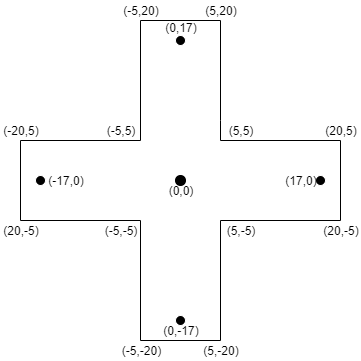
\includegraphics [width=0.5\columnwidth]{bab2/img/contoh-kasus-tanpa-solusi}
	\caption {Ilustrasi contoh kasus tanpa solusi}
	\label {fig:ilustrasi-contoh-kasus-tanpa-solusi}
\end{figure}
\begin{figure}
	\Centering
	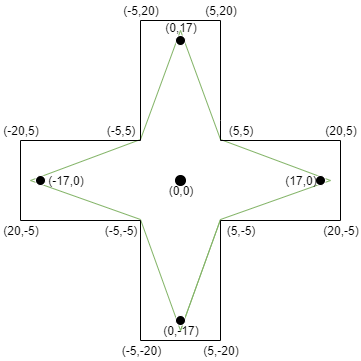
\includegraphics [width=0.5\columnwidth]{bab2/img/contoh-kasus}
	\caption {Ilustrasi contoh kasus}
	\label {fig:ilustrasi-contoh-kasus}
\end{figure}

\section{Strategi Penyelesaian Permasalahan}
Pada buku ini membatasi hanya untuk poligon sederhana. Titik yang berada di dalam poligon dapat diganti dengan poligon sederhana, segment garis atau yang lainnya.
\par Asumsikan poligon $A$ mempunyai $n$ vertex, dimana $A = \left \langle p_1, p_2, ..., p_n \right \rangle$. Poligon $A$ merupakan poligon yang membatasi kumpulan titik $S$ yang mempunyai titik sebanyak $m$ ($S = \left \langle q_1, q_2, ..., q_m \right \rangle$). $P(A)$ merupakan sebuah deque yang menampung vertex dari poligon $A$.
\par untuk setiap 